\documentclass{article}

\usepackage{repsty}

\newcommand{\Tint}{\Delta t}
\DeclareDocumentCommand{\v}{O{}mo}{\sigma^2_{#1}\bkt*{#2\IfValueT{#3}{|~ #3}}}
\DeclareDocumentCommand{\Xpct}{O{}mo}{\mathrm{E}_{#1}\bkt*{#2\IfValueT{#3}{|~ #3}}}


\begin{document}
	
\title{Beam current resolution}
\author{Alexander Aksentyev}
\maketitle
	
In the transmission-experiment method of determining a double-polarized observable, one estimates the beam's rate of decay by fitting a linear model to the log-transformed beam current measurements:
\begin{align*}
	\tilde{I}_t  &= I_0 \cdot e^{-\nu\CS\Thick\cdot t} + \err^I_t = I_t + \err^I_t, \\
	\ln \tilde{I}_t &= \ln I_0 + \slp t + \delta^I_t,
\end{align*}
	where $\nu$ is the circulation frequency, $\CS = \CS[0]\bkt{1 + \A P^b_y P^t_{xz} + A_{y,y} P^b_y P^t_y + \dots}$ is the total scattering cross section, $\Thick$ is the target thickness, $\err^I_t$ is the measurement error at time $t$, $I_t$ is the actual beam current, $\tilde{I}_t$ is the measured beam current, and $\delta^I_t = \sfrac{\err^I_t}{I_t}$.


The observable $\A$ can then be estimated as a difference statistic of the slopes from a pair of appropriate polarization cases: $\A* = C\bkt*{\slp*^- - \slp*^+}$, $C = \bkt{\nu\CS[0]\Thick P^b_y P^t_{xz}}^{-1}$, and its variance will be proportional to the sum of the variances of the constituent slope estimates: $\SE{\A*} = C\sqrt{2}\cdot\SE{\slp*}$.

For the mean statistic, its precision depends on the precision of the slope estimate $\SE{\slp*}$ as in
\begin{equation}\label{eq:AvgASE}
\SE{\avg{\A*}} = \frac{\SE{\A*}}{\sqrt N} = \sqrt{2}\sqrt{\frac hH}\cdot\SE{\A*} = 2C\sqrt{\frac hH}\cdot\SE{\slp*},
\end{equation}
where $H$ is the beam time, $h$ the cycle length, and so the maximum number of estimate pairs $N = \sfrac{H}{2h}$.

Under the Gauss-Markov conditions, the Ordinary Least Squares estimator of the slope is zero-bias, minimum-variance, and has a standard error of
\begin{equation}\label{eq:SlpVarGM}
\SE{\slp*} = \frac{\SE{\delta^I}}{\sqrt{\sum_{k=1}^K (t_k - \avg{t})^2}},
\end{equation}
where $\SE{\delta^I}$ is termed the beam current resolution, $K$ is the sample size, and $t_k$ is the measurement time. For samples taken uniformly in time with step $\Tint$, at sample sizes $K = h/\Tint \gg 1$, the denominator can be expressed in physical terms as
\[
\sqrt{\sum_{k=1}^K (t_k - \avg{t})^2} \approx \frac{h\sqrt{h}}{2\sqrt{3}\sqrt{\Tint}},
\]
and hence 
\begin{equation}\label{eq:SlpVar}
	\SE{\slp*} = 2\sqrt{3}\sqrt{\frac{\Delta t}{h}}\frac{\SE{\delta^I}}{h},
\end{equation}
\begin{equation}
	\SE{\avg{\A*}} = 4\sqrt{3}C\cdot \frac{\sqrt{\Tint}}{h\sqrt{H}}\cdot\SE{\delta^I},
\end{equation}
from which the required measurement resolution can be estimated for the given precision $\SE{\avg{\A*}}$, beam time $H$, and cycle duration $h$.

\begin{table}[h]
	\centering
	\caption{Parameter values (June 2016)\label{tbl:Param}}
	\begin{threeparttable}[h]
		\begin{tabular}{p{4.5cm}llr}
			\hline\hline
			Parameter                                      & Symbol            & Value              &               Dimension \\ \hline
			Beam revolution frequency                      & $\nu$             & 0.79               &                     MHz \\
			Target thickness                               & $\Thick$          & $1.1\cdot 10^{14}$ & $\Dim{at\cdot cm^{-2}}$ \\
			Target polarization                            & $P^t$             & 0.88               &                      -- \\
			Beam polarization                              & $P^b$             & 0.74               &                      -- \\
			$pd$ scattering cross section                  & $\CS[0]$\tnote{a} & 70                 &                      mb \\
			Slope-to-Asymmetry proportionality coefficient & $C$               & $1.26\cdot 10^5$   &                     sec \\ \hline
		\end{tabular}
		\begin{tablenotes}
			\item[a]{From Particle Data Group \url{http://pdg.lbl.gov/2016/hadronic-xsections/rpp2014-pd_pn_plots.pdf}}
		\end{tablenotes}
	\end{threeparttable}
\end{table}

\section{Resolution lower bound}
If, during measurement, the beam current slope varies (due to such factors as the variation of the target thickness, or drifting current transformer offset), that variation will influence the standard error of the estimate in accordance with the law of total variance:
\begin{equation}\label{eq:VarSlpLTV}
\v{\slp*} = \Xpct[\slp]{\v{\slp*}[\slp]} + \v[\slp]{\Xpct{\slp*}[\slp]}.
\end{equation}
Here, 
\begin{align}
\Xpct{\slp*}[\slp] 	&= \slp, \notag\\
\v{\slp*}[\slp] 	&= 12\frac{\Tint}{h}\frac{\v{\delta^I}}{h^2}, \tag{eq.~\eqref{eq:SlpVar}}
\shortintertext{and hence}
\v{\avg{\A*}}		&= \frac{4 C^2}{H}\bkt{12\Tint\cdot\frac{\v{\delta^I}}{h^2} + h\cdot\v{\slp}}.\label{eq:SEA}
\end{align}

In the last equation, the first term describes the statistical precision of the estimate, the second its accuracy. The accuracy term constrains our ability to improve precision by reducing measurement resolution; this can be observed in Figure~\ref{fig:SEA_varb}.

\begin{figure}[h]
	\centering
	\begin{minipage}{.5\textwidth}
		\centering
		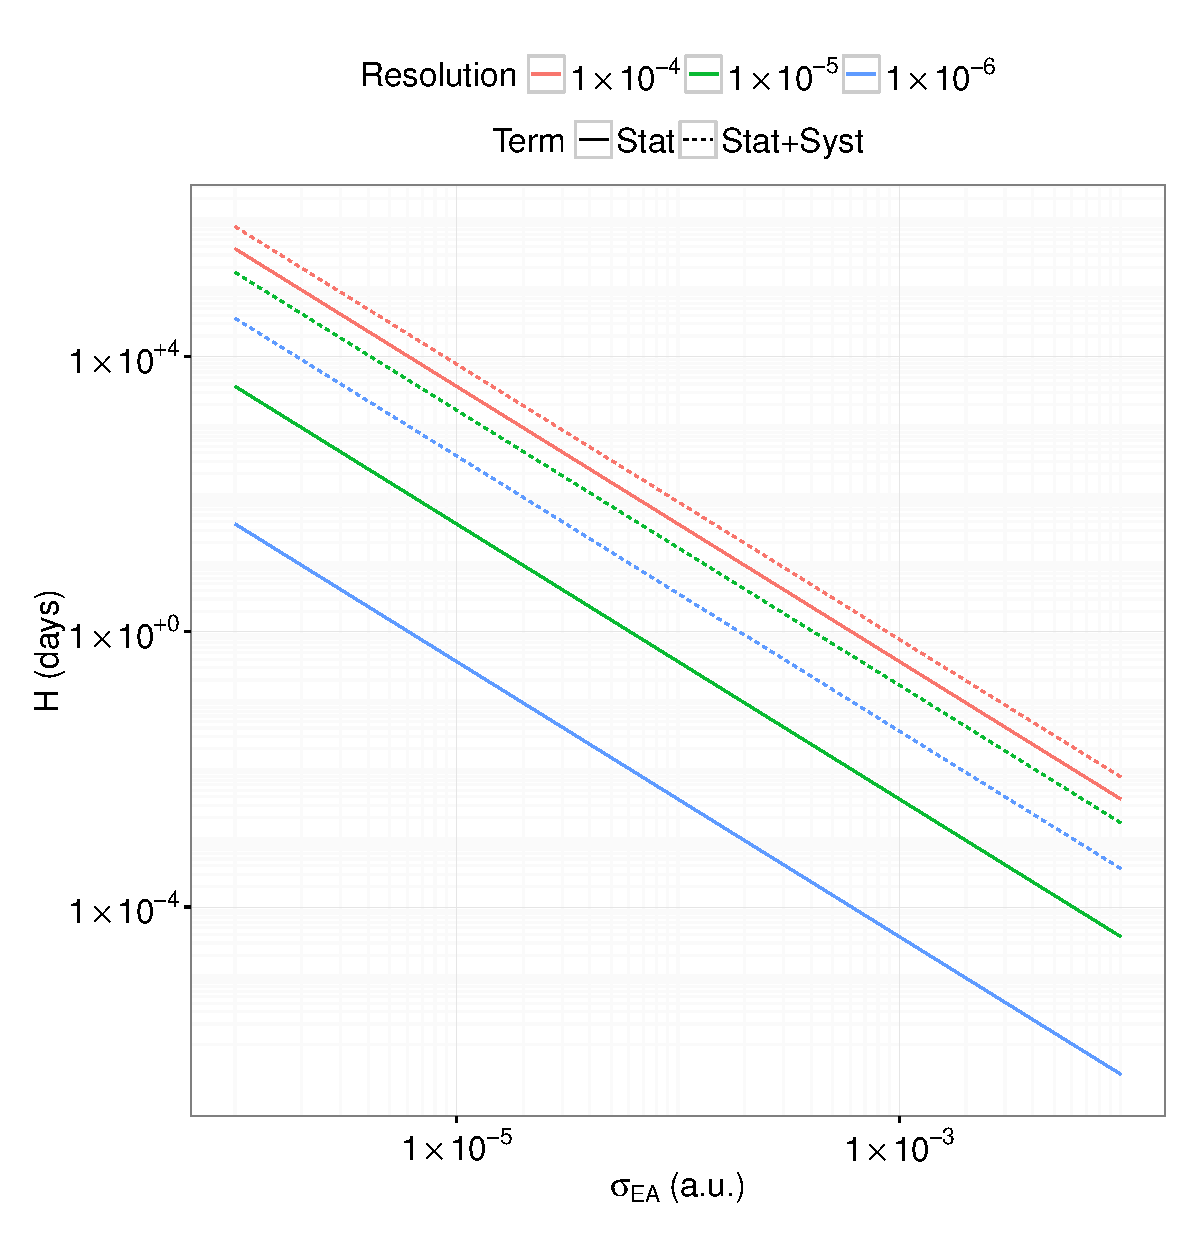
\includegraphics[scale=.5]{Polish_BeamTime_Plot.eps}
		\caption{Required beam time as a function of figure-of-merit precision, when the inherent slope variation $\v{\slp} = 0$ (continuous lines), and $\v{\slp} =  10^{-15}$ (dashed lines), for different levels of beam current resolution. The dashed lines' values are computed at the optimal cycle durations.}
	\end{minipage}~~
	\begin{minipage}{.5\textwidth}
		\centering
		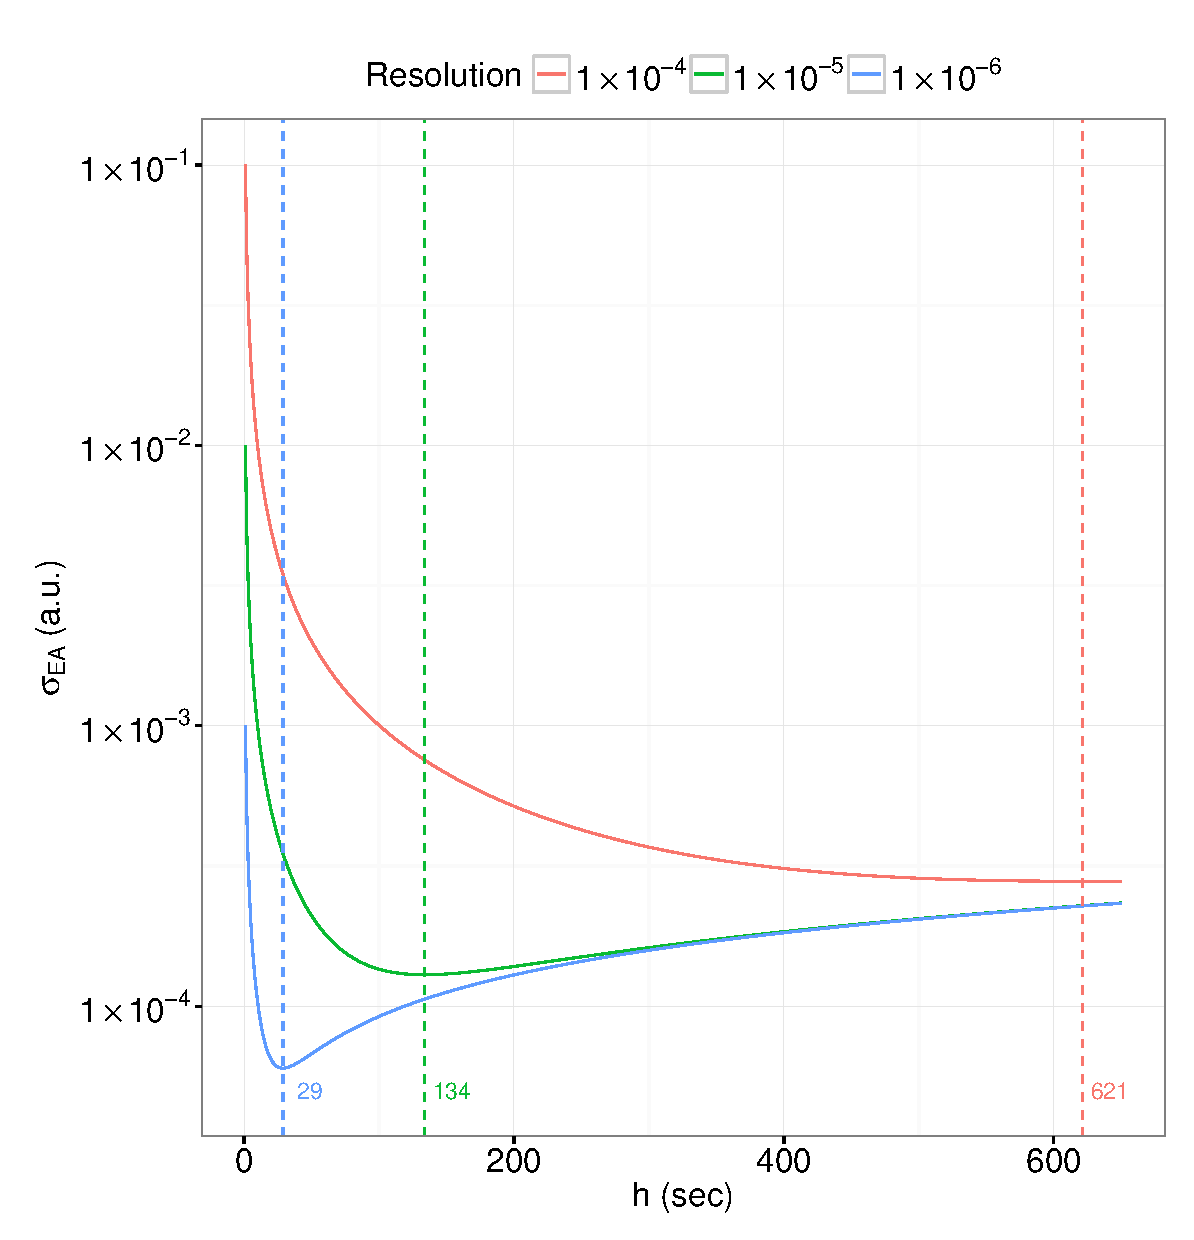
\includegraphics[scale=.5]{Polish_StateTime_Plot.eps}
		\caption{The standard error of the mean $\A$ estimate as a function of cycle length when the inherent slope variation $\v{\slp} = 10^{-15}$. The inherent variation limits the accuracy of the estimate.\label{fig:SEA_varb}}
	\end{minipage}
\end{figure}

From equation~\eqref{eq:SEA}, the best variance is achieved at
\begin{equation}
h_{best} = \sqrt[3]{24\cdot \Tint} \bkt{\frac{\v{\delta^I}}{\v{\slp}}}^{1/3}.
\end{equation}
In Table~\ref{tbl:SEA_varb}, cycle durations for the given values of $\v{\slp} = 10^{-15}$ sec$^{-2}$ and $\SE{\delta^I}$ are summarized.
\begin{table}[h]
	\centering
	\caption{Best achievable precision of $\A*$,\\ and the corresponding cycle time\\ for a given resolution.\label{tbl:SEA_varb}}
	\begin{tabular}{lrr}
		\hline\hline
		$\SE{\delta^I}$ & $h_{best}$ (sec) & $\SE{\avg{\A*}}$ \\ \hline
		$1\cdot10^{-4}$ &              621 &  $2.8\cdot10^{-4}$ \\
		$1\cdot10^{-5}$ &              134 &  $1.3\cdot10^{-4}$ \\
		$1\cdot10^{-6}$ &               29 &  $6.0\cdot10^{-5}$ \\ \hline
	\end{tabular}
\end{table}

	
\end{document}